\section*{Problem 1}
\subsection*{Part a}
The atom is face centered cubic.
\subsection*{Part b}
If we pick one of the corner Zn atoms to be the origin then we can describe every other atom with a basis vectors $a_1 = \frac{1}{4} (1,0,0)$, $a_2 = \frac{1}{4} (0,1,0)$, and $a_3 = \frac{1}{4} (0,0,1)$.
\subsection*{Part c}
Given $a = 0.541nm$ the spacing between the nearest Zn atoms is $\Delta (Zn-Zn) = \frac{1}{2} a \approx 0.271nm$. The spacing $\Delta (Zn-S) = \sqrt{(\frac{1}{4}a)^2+(\frac{1}{4}a)^2} = a \frac{\sqrt{2}}{4} \approx 0.191nm$. The spacing $\Delta (S-S) = \sqrt{(\frac{1}{2}a)^2 + (\frac{1}{2}a)^2} = a \frac{\sqrt{2}}{2} \approx 0.383nm$.

\pagebreak
\section*{Problem 2}
\subsection*{Part a}
Restating Eq 13.3 let $f = (a_i)$ be a basis, then there exists a unique basis called the reciprocal basis $f^\# = (b_i)$ such that
\eq{
\Vec{a_i}\cdot \Vec{b_j} &= \gamma \delta_{ij}
}
for some $\gamma \in \mathbb{R}$. Geometrically, this means that if $A$ is a map $f \rightarrow f^\#$, then we decompose it into a scaling by $\gamma$ and a rigid rotation by $B$ that cycles the basis vectors, ie $B\Vec{a}_i = \Vec{a}_{i+1}$. Since $B$ is a orthogonal transformation we can write
\eq{
A &= \gamma B\\
AB^{-1} &= \gamma I\\
AB^T &= \gamma I
}
and we can of course choose $\gamma = 2\pi$.

We can write the basis vectors $\Vec{b}_i \in f^\#$ in the $f$ basis, where
\eq{
\Vec{b}_i = b_{i1}\Vec{a}_1 + b_{i2}\Vec{a}_2 + b_{i3}\Vec{a}_3
}
then we know from linear algebra that the rows of $A$ will be the coefficients, ie
\eq{
A &= \begin{bmatrix}
    b_{11} & b_{12} & b_{13}\\
    b_{21} & b_{22} & b_{23}\\
    b_{31} & b_{32} & b_{33}\\
\end{bmatrix}
}
Similarly
\eq{
B &= \begin{bmatrix}
    0 & 0 & 1\\
    1 & 0 & 0\\
    0 & 1 & 0\\
\end{bmatrix}^k\\
}
Where $k = 0,1,2$. Geometrically the rows of $B$ are the coefficients of the rotation transformation from the $f$ to $f^\#$ basis, and so the columns of $B^T$ are the same thing.

\subsection*{Part b}
Starting with the basis vectors in SSB, we can easily reduce them
\pagebreak
\section*{Problem 3}
\subsection*{Part a}
The primitive lattice vectors are
\eq{
\Vec{a}_1 &= a \hat{x}\\
\Vec{a}_2 &= \frac{a}{2}\hat{x} + \frac{a\sqrt{3}}{2}\hat{y}\\
\Vec{a}_3 &= c\hat{z}
}
So the reciprocal lattice vectors are
\eq{
\Vec{b}_1 &= 2\pi\frac{\Vec{a}_2\times\Vec{a}_3}{\Vec{a}_1\cdot(\Vec{a}_2\times\Vec{a}_3)}\\
&= \frac{2\pi}{a}\hat{x}-\frac{2\pi}{a\sqrt{3}}\hat{y}\\
\Vec{b}_2 &= \frac{4\pi}{a\sqrt{3}}\hat{x}\\
\Vec{b}_3 &= \frac{2\pi}{c}\hat{z}
}

\subsection*{Part b}
The volume is given by
\eq{
V &= \det{\begin{bmatrix}
    b_{1x} & b_{1y} & b_{1z}\\
    b_{2x} & b_{2y} & b_{2z}\\
    b_{3x} & b_{3y} & b_{3z}\\
\end{bmatrix}}\\
&= -b_{1y}b_{3z}b_{2x}\\
&= \frac{16 \pi^3}{3}\frac{1}{a^2 c}
}
\subsection*{Part c}
We'll compute $|G_{hkl}|^2$ first
\eq{
|G_{hkl}|^2 &= |h\Vec{b}_1 + k\Vec{b}_2 + l\Vec{b}_3|^2\\
&= |(2\pi)((\frac{h}{a}+\frac{2k}{a\sqrt{3}})\hat{x}+(\frac{h}{a\sqrt{3}})\hat{y}+(\frac{l}{c})\hat{z})|^2\\
&= (2\pi)^2((\frac{h}{a}+\frac{2k}{a\sqrt{3}})^2+(\frac{h}{a\sqrt{3}})^2+(\frac{l}{c})^2)
}
The spacing is
\eq{
d_{hkl} &= \frac{2\pi}{|G_{hkl}|}\\
&= ((\frac{h}{a}+\frac{2k}{a\sqrt{3}})^2+(\frac{h}{a\sqrt{3}})^2+(\frac{l}{c})^2)^{-\frac{1}{2}}
}
\pagebreak
\section*{Problem 4}
The angle between the red and black lattice is $\arctan(\frac{1}{2})$. In this case, the new smallest repeating pattern which tiles the plane is the unit cell defined by the red lattice.

To generate the new lattice basis we rotate our original frame by $\arctan(\frac{1}{2})$ and stretch it by $\sqrt{5}$, which we can denote by the matrix transformation $\sqrt{5}R$.

Then $\Vec{n} = \sqrt{5}R\Vec{a_1}$ and $\Vec{m} = \sqrt{5}R\Vec{a_2}$ since rigid rotations preserve length we know that
\eq{
\Vec{n}\times \Vec{m} &= \sqrt{5}R\Vec{a_1} \times \sqrt{5}R\Vec{a_2}\\
&= 5|\Vec{a_1}||\Vec{a_2}|(\hat{a_1}\times\hat{a_2})\\
&= 5a^2\hat{a_3}
}
Where $\hat{a}_3$ is just some unit vector normal to the plane. This is the result we expect since the super lattice is a square with side length $\sqrt{5}a$. Using the provided notation we can describe the new super lattice as
\eq{
(\Vec{n}\times\Vec{m})R\theta = (\sqrt{5} \times \sqrt{5})R\arctan(\frac{1}{2})
}
\pagebreak
\section*{Problem 5}
\subsection*{Part a}
The false color plot is below
\begin{figure}[H]
    \centering
    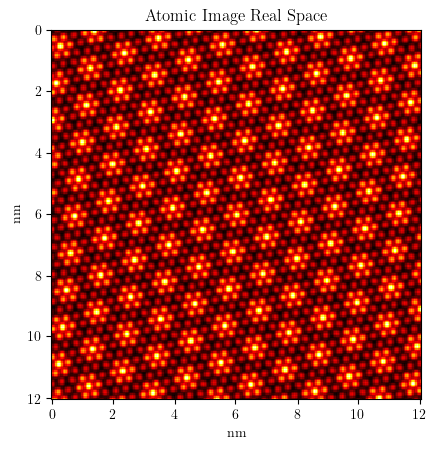
\includegraphics[width=0.75\linewidth]{Resources//140A//Homework 6/140A Homework 6 Problem 5a.png}
    \label{fig:enter-label}
\end{figure}
Zooming in we can see that the spacing between repeating units is $a\approx 0.32nm$ and the wavelength of the CDW is $\lambda \approx 1.2nm \approx 3.8a$. The primitive lattice and CDW appears rhombohedral.
\subsection*{Part b}
Here we've plotted a zoomed in version of the atomic lattice so we can plot the primitive lattice and super lattice vectors.
\begin{figure}[H]
    \centering
    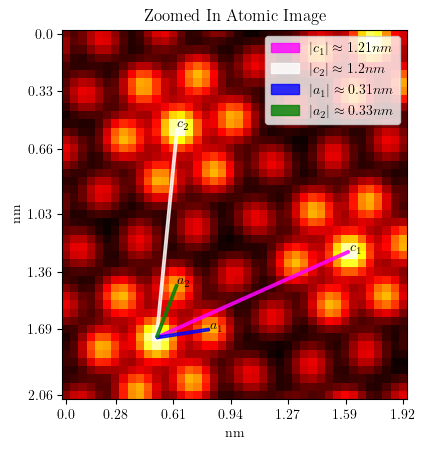
\includegraphics[width=1\linewidth]{Resources//140A//Homework 6/140A Homework 6 Problem 5b.png}
    \caption{Plot of lattice vectors, with their magnitudes in the top right.}
    \label{fig:enter-label}
\end{figure}

\subsection*{Part c}
Using the basis vectors from part b we compute the reciprocal vectors and can see where each of the Bragg peaks for the atomic lattice line up.
\begin{figure}[H]
    \centering
    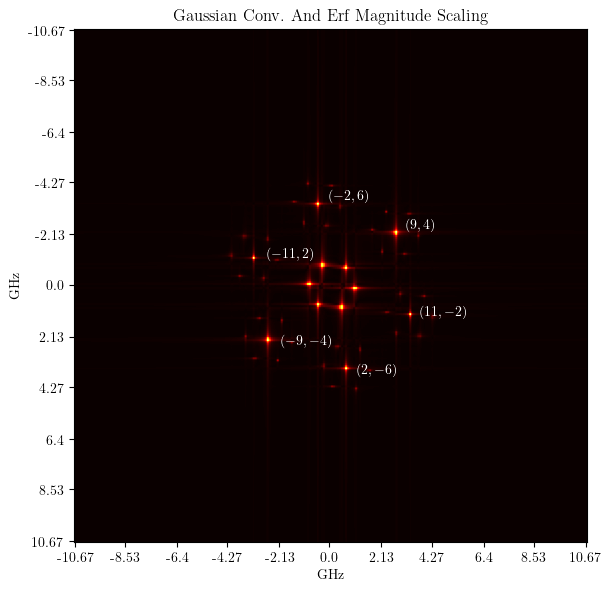
\includegraphics[width=1\linewidth]{Resources//140A//Homework 6/140A Homework 6 Problem 5c.png}
    \caption{Spectral power plot, in units of linear spatial frequency. The annotated Bragg peaks are those that correspond to the atomic lattice.}
    \label{fig:enter-label}
\end{figure}
The output of the fft was shifted so the DC component (which was removed) is at the center. The image was passed through a Gaussian filter to increase the spot size, then passed through the error function to provide a non-linear gain to the darker peaks.
\subsection*{Part d}
The Brillouin zone is any primitive cell of the reciprocal lattice. In real space the CDW lattice is larger, by a factor of about 3, than the atomic lattice. So in reciprocal space we expect a primitive cell that is about 3 times smaller. This leads to a shrinking of the Brillouin zone, so we expect "folding" around the atomic lattice points.

\pagebreak
\section*{Appendix}
\subsection*{Problem 5}
\subsubsection*{Part a}
\begin{python}
import numpy as np
import matplotlib.pyplot as plt
from scipy.ndimage import gaussian_filter
from scipy.special import erf

# Part a
with open('HW6_STM_256x256_12nm.txt') as f:
    lines = f.readlines()
lines = np.array([list(map(lambda n: float(n), line.split())) for line in lines])

# Plot heat map
plt.rcParams.update({
    "text.usetex": True,
    "font.family": "Serif"
})
point_labels = np.linspace(0,12,7,dtype=int)
points = np.linspace(0,255,7,dtype=int)
plt.imshow(lines, cmap='hot', interpolation='nearest')

plt.xticks(points,point_labels)
plt.yticks(points,point_labels)

plt.xlabel("nm")
plt.ylabel("nm")

plt.title("Atomic Image Real Space")

plt.show()
\end{python}
\subsubsection*{Part b}
\begin{python}
# Part b
plt.imshow(lines[15:60,13:55], cmap='hot', interpolation='nearest')

pointsx = np.linspace(0,55-13-1,7,dtype=int)
pointsxlabels = np.round(pointsx*(12/256),2)

pointsy = np.linspace(0,60-15-1,7,dtype=int)
pointsylabels = np.round(pointsy*(12/256),2)

originx = 11
originy = 37

c1 = [23.5, -10.5]
plt.arrow(originx, originy,c1[0],c1[1], width=0.3,
    head_width=0.08,
    head_length=0.1,
    color=('magenta',0.8),
    length_includes_head=True)
plt.text(originx + c1[0],originy+c1[1], "$c_1$")

c2 = [2.5,-25.5]
plt.arrow(originx, originy,c2[0],c2[1], width=0.3,
    head_width=0.08,
    head_length=0.1,
    color=('white',0.8),
    length_includes_head=True)
plt.text(originx + c2[0], originy + c2[1], "$c_2$")

a1 = [6.5,-1]
plt.arrow(originx, originy, a1[0], a1[1], width=0.3,
    head_width=0.08,
    head_length=0.1,
    color=('blue',0.8),
    length_includes_head=True)
plt.text(originx + a1[0], originy + a1[1], "$a_1$")

a2 = [2.5, -6.5]
plt.arrow(originx, originy, a2[0], a2[1], width=0.3,
    head_width=0.08,
    head_length=0.1,
    color=('green',0.8),
    length_includes_head=True)
plt.text(originx + a2[0], originy + a2[1], "$a_2$")

plt.title("Zoomed In Atomic Image")
plt.yticks(pointsy, pointsylabels)
plt.xticks(pointsx, pointsxlabels)
plt.xlabel("nm")
plt.ylabel("nm")
plt.legend(["$|c_1| \\approx "+str(round(np.sqrt(c1[0]**2+c1[1]**2)*(12/256),2))+"nm$",
            "$|c_2| \\approx "+str(round(np.sqrt(c2[0]**2+c2[1]**2)*(12/256),2))+"nm$",
            "$|a_1| \\approx "+str(round(np.sqrt(a1[0]**2+a1[1]**2)*(12/256),2))+"nm$",
            "$|a_2| \\approx "+str(round(np.sqrt(a2[0]**2+a2[1]**2)*(12/256),2))+"nm$"])

plt.show()
\end{python}
\subsubsection*{Part c}
\begin{python}
# Part c
sample_length = 12 #nm
fmax = 256/sample_length

b1 = [2*np.pi/a for a in a1]
b2 = [2*np.pi/a for a in a2]

fpoints = np.round(np.linspace(0,fmax,11)-fmax/2,2)
findicies = np.linspace(0,255,11,dtype=int)

# Average to remove DC bias
avg = np.mean(np.ndarray.flatten(lines))
# Compute 2D DFT
spec = np.absolute(np.fft.fftshift(np.fft.fft2(lines-avg)))

# Filter data to see points better
specfilt = gaussian_filter(spec, sigma=0.1)
specfiltnorm = erf(np.absolute(specfilt)/max(np.ndarray.flatten(np.absolute(specfilt)))*2)

# Plot data
plt.close('all')
fig1 = plt.figure(figsize=(6, 6), layout="constrained")
gs1_main = fig1.add_gridspec(1,1)

ax1 = fig1.add_subplot(gs1_main[0])
ax1.imshow(specfiltnorm, cmap='hot')
ax1.set_title("Gaussian Conv. And Erf Magnitude Scaling")
ax1.set_yticks(findicies,fpoints)
ax1.set_ylabel("GHz")
ax1.set_xticks(findicies,fpoints)
ax1.set_xlabel("GHz")

indexo = [128,128]
text_offsetx = 6

h = 9
k = 4
ax1.text(indexo[0]+h*(b1[0]+b2[0])+text_offsetx,indexo[1]+k*(b1[1]+b2[1]),"$(9,4)$",color=('white',1))
ax1.text(indexo[0]-h*(b1[0]+b2[0])+text_offsetx,indexo[1]-k*(b1[1]+b2[1]),"$(-9,-4)$",color=('white',1))

h = -2
k = 6
ax1.text(indexo[0]+h*(b1[0]+b2[0])+text_offsetx,indexo[1]+k*(b1[1]+b2[1]),"$(-2,6)$",color=('white',1))
ax1.text(indexo[0]-h*(b1[0]+b2[0])+text_offsetx,indexo[1]-k*(b1[1]+b2[1]),"$(2,-6)$",color=('white',1))

h = -11
k = 2
ax1.text(indexo[0]+h*(b1[0]+b2[0])+text_offsetx,indexo[1]+k*(b1[1]+b2[1]),"$(-11,2)$",color=('white',1))
ax1.text(indexo[0]-h*(b1[0]+b2[0])+text_offsetx,indexo[1]-k*(b1[1]+b2[1]),"$(11,-2)$",color=('white',1))

plt.show()
\end{python}